\chapter{Continuum approach}
\section{Identical sinks}

The distribution of the concentration \(C(x)\) of a solute in a constant,
uniform, unidirectional flow \(u_0\) in a domain of length \(L\) containing
\(N\) identical point sinks of constant strength \(q_0\) is governed by the
one-dimensional advection-diffusion equation,
\begin{subequations}
    \label{eqn:nondim_advec_diff}
    \begin{gather}
        \label{eqn:nondim_advec_diff_eq}
        \Pe C_x - C_{xx} = - \Da f(x), \text{ for } 0 < x < \varepsilon^{-1},\\
        \label{eqn:nondim_advec_diff_bcs}
        C(0) = 1, \quad C(\varepsilon^{-1}) = 0,
    \end{gather}
\end{subequations}
where \(\Pe=u_0 l/D\) is the Péclet number, \(\Da=q_0 l/(D C_0)\) is the
Damköhler number and the sink distribution is given by
\begin{equation}
    \label{eqn:point_sink_dist}
    f(x) = \sum_{i=1}^{N} \delta(x-\xi_i).
\end{equation}
The ordered sink locations \(0 < \xi_1 < \cdots < \xi_N < L\) must be sampled
from a distribution, either a periodic distribution, i.e. \(\xi_i=i,
\Delta_i=1\), where \(\Delta_i = \xi_i - \xi_{i-1}\), for \(1\le\xi\le N\), or
some random distribution (TODO). For convenience, define \(\xi_0 = 0\) and
\(\xi_{N+1} = \varepsilon^{-1}\).

Regardless of the distribution of the sink locations, the solution between any
two sinks (including the boundary points \(\xi_0, \xi_{N+1}\)), say \(\xi_i,
\xi_{i+1}\), is of the following form,
\begin{gather}
    \label{eqn:gen_sol_piece}
    C_i(x)=A_i e^{\Pe x}+B_i\\
    \text{ for } \xi_i \le x \le \xi_{i+1}, \text{ for } 0 \le i \le N.
\end{gather}

To determine the constants \(A_i, B_i\), we must apply the boundary conditions
of the problem to the general solution.

The boundary conditions~\eqref{eqn:nondim_advec_diff_bcs} imply
\begin{equation}
    \label{eqn:bc_A_0_B_0}
    C_0(0) = A_0 + B_0 = 1,
\end{equation}
and
\begin{equation}
    \label{eqn:bc_A_N_B_N}
    C_N(1) = A_N e^{\Pe} + B_N = 0.
\end{equation}

However, to fully determine the coefficients we must first obtain the
conditions on the flux of concentration at the locations of the sinks. To do
this for the sink at \(\xi_i\), say, we integrate
equation~\eqref{eqn:nondim_advec_diff_eq} over the interval
\([\xi_i-\alpha,\xi_i+\alpha]\), and take the limit as \(\alpha \to 0\):
\begin{align*}
    \lim_{\alpha \to 0}
    \int_{\xi_i-\alpha}^{\xi_i+\alpha}\left(\Pe C_x - C_{xx}\right)\dd x = &
    \lim_{\alpha \to 0}
    \Big[\Pe C - C_x\Big]_{\xi_i-\alpha}^{\xi_i+\alpha}\\
    = & C_x^-(\xi_i) - C_x^+(\xi_i)\\
    = & -\lim_{\alpha \to 0}
    \int_{\xi_i-\alpha}^{\xi_i+\alpha}\Da f(x) \dd x\\
    = & - \Da,
\end{align*}
where we have applied the condition that the concentration \(C(x)\) is
continuous everywhere, and standard properties of the Dirac delta function.
Therefore, the flux of the concentration decreases by the Damköhler
number \(\Da\) at each sink.

We can then apply the flux condition to equation~\eqref{eqn:gen_sol_piece} for
the two pieces of the solution that meet at the sink at \(\xi_i\):
\(C_{i-1}(x)\) and \(C_i(x)\).
\begin{equation*}
    %\nonumber
    {C_{i-1}}_x(\xi_i) = {C_i}_x(\xi_i) - \Da,%\\
    %\nonumber
    %\implies & \Pe A_{i-1} e^{\Pe \xi_i} = \Pe A_i e^{\Pe \xi_i} - \Da\\
\end{equation*}
which gives after substitution
\begin{equation}
    \label{eqn:bc_A_i}
    A_i = A_{i-1} + \frac{e^{-\Pe \xi_i}\Da}{\Pe}.
\end{equation}
Applying \eqref{eqn:bc_A_i} to itself recursively gives an expression for
\(A_i\) in terms of the sinks locations and \(A_0\):
\begin{equation}
    \label{eqn:A_i}
    %\boxed{
    A_i = A_0 + \frac{\Da}{\Pe}\sum_{j=1}^{i} e^{-\Pe \xi_j}
    %}
\end{equation}
Similarly, continuity of concentration across the sink at \(\xi_i\) gives
\begin{equation*}
    %\nonumber
    C_{i-1}(\xi_i) = C_i(\xi_i),
\end{equation*}
and so
\begin{equation}
    %\nonumber
    %\implies & A_{i-1} e^{\Pe \xi_i} + B_{i-1} = A_i e^{\Pe \xi_i} + B_i\\
    %\nonumber
    %\implies & A_{i-1} e^{\Pe \xi_i} + B_{i-1} = \frac{\Da}{\Pe} + A_{i-1}
    %e^{\Pe \xi_i} + B_i\\
    \label{eqn:bc_B_i}
    B_i = B_{i-1}-\frac{\Da}{\Pe}.
\end{equation}
As above, applying \eqref{eqn:bc_B_i} recursively gives an expression for
\(B_i\):
\begin{equation}
    \label{eqn:B_i}
    %\boxed{
    B_i = B_0 - i\frac{\Da}{\Pe}.
    %}
\end{equation}
Applying \eqref{eqn:bc_B_i} to \eqref{eqn:bc_A_0_B_0} \(N\) times gives
\begin{equation}
    \label{eqn:bc_A_0_B_N}
    A_0 + N \frac{\Da}{\Pe} + B_N = 1.
\end{equation}
Now use \eqref{eqn:bc_A_N_B_N} with \eqref{eqn:bc_A_0_B_N} to obtain
\begin{equation}
    \label{eqn:bc_A_0_A_N}
    A_0 + N \frac{\Da}{\Pe} - A_N e^{\Pe \varepsilon^{-1}} = 1.
\end{equation}
Applying \eqref{eqn:bc_A_i} to \eqref{eqn:bc_A_0_A_N} \(N\) times and
rearranging gives
\begin{equation}
    %\nonumber
    %& A_0 + N \frac{\Da}{\Pe} - e^{\Pe \varepsilon^{-1}}
    %\left(A_0 + \frac{\Da}{\Pe} \sum_{i=1}^{N}e^{-\Pe \xi_i}\right) = 1\\
    %\nonumber
    %\implies & \left(1 - e^{\Pe \varepsilon^{-1}}\right) A_0 +
    %\frac{\Da}{\Pe} \left(N - e^{\Pe \varepsilon^{-1}} \sum_{i=1}^{N} e^{-\Pe
    %\xi_i}\right) = 1\\
    %\implies & \boxed{
    \label{eqn:A_0}
    A_0 = \frac{1 -
    \frac{\Da}{\Pe} \left(N - e^{\Pe \varepsilon^{-1}} \sum_{i=1}^{N} e^{-\Pe
    \xi_i}\right)}{1 - e^{\Pe \varepsilon^{-1}}}.
    %}
\end{equation}
Similarly, \eqref{eqn:A_0} and \eqref{eqn:bc_A_0_B_0} give
\begin{equation}
    %\boxed{
    \label{eqn:B_0}
    B_0 = 1 - \frac{1 -
    \frac{\Da}{\Pe} \left(N - e^{\Pe \varepsilon^{-1}} \sum_{i=1}^{N} e^{-\Pe
    \xi_i}\right)}{1 - e^{\Pe \varepsilon^{-1}}}.
    %}
\end{equation}

\begin{figure}[ht!]
    \centering
    \begin{subfigure}[b]{0.45\textwidth}
        \centering
        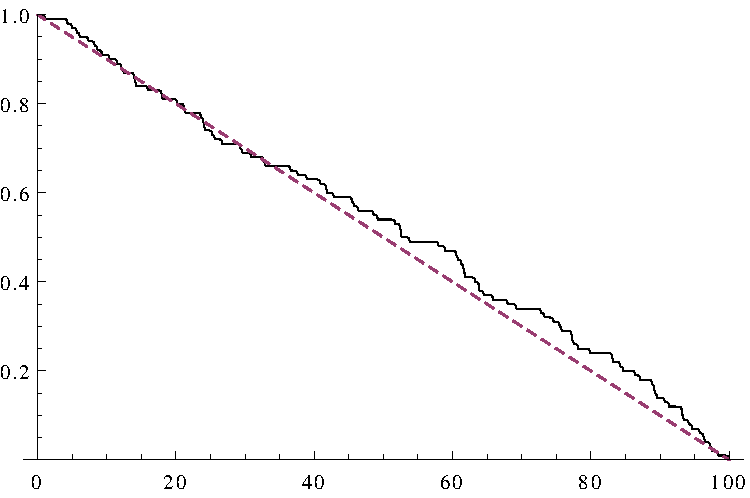
\includegraphics[scale=0.5]{continuum/figures/loc_uniform_dist/1}
    \end{subfigure}
    \begin{subfigure}[b]{0.45\textwidth}
        \centering
        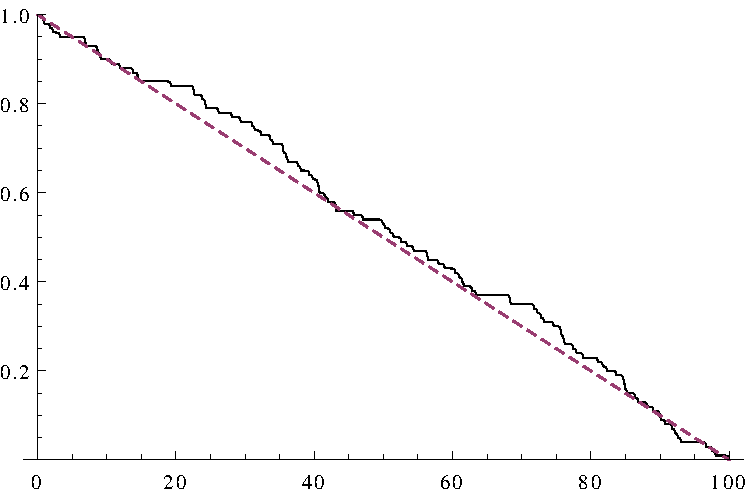
\includegraphics[scale=0.5]{continuum/figures/loc_uniform_dist/2}
    \end{subfigure}
    \\
    \begin{subfigure}[b]{0.45\textwidth}
        \centering
        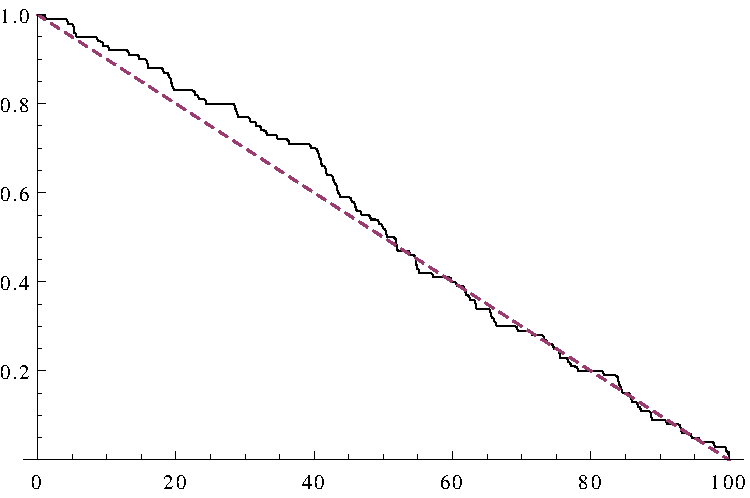
\includegraphics[scale=0.5]{continuum/figures/loc_uniform_dist/3}
    \end{subfigure}
    \begin{subfigure}[b]{0.45\textwidth}
        \centering
        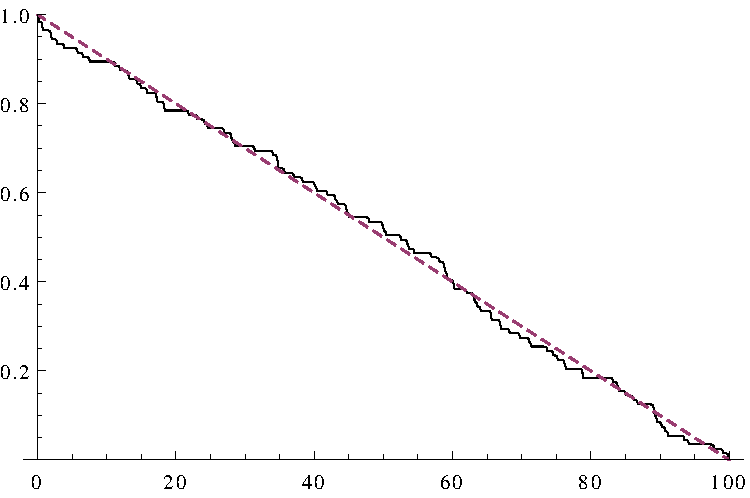
\includegraphics[scale=0.5]{continuum/figures/loc_uniform_dist/4}
    \end{subfigure}
    \caption{\label{fig:99_sinks_uni_pos}Four realisations of 99 sinks with
    uniformly random positions and
        \({\Pe=10}, {\Da=\varepsilon\Pe}\)}
\end{figure}

\FloatBarrier

\subsubsection{Sample statistics}
We define the homogenisation residue as
\begin{equation}
    \label{eqn:homogenisation_residue}
    r^\varepsilon(X) = C - C^{(0)}.
\end{equation}

In the regime \(\Pe = \bo{\varepsilon}, \Da = \bo{\varepsilon^2}\), the
first order homogenisation approximation is \(C^{(0)}(X) = 1 - X\). We will use
the residue to compare realisations of concentration distributions to the first
order approximation.

Figure~\ref{fig:loc_uniform_1000_av_residuals} shows the sample mean and
variance (scaled by a factor of \(\varepsilon^{-1}\) *is there a mathematical
reason for the scalings in the papers or are they graphically convenient? This
one is the latter\ldots*) of
\(r^\varepsilon\) computed from 1000 realisations of the uniformly random sink
locations.

\begin{figure}[ht!]
    \centering
    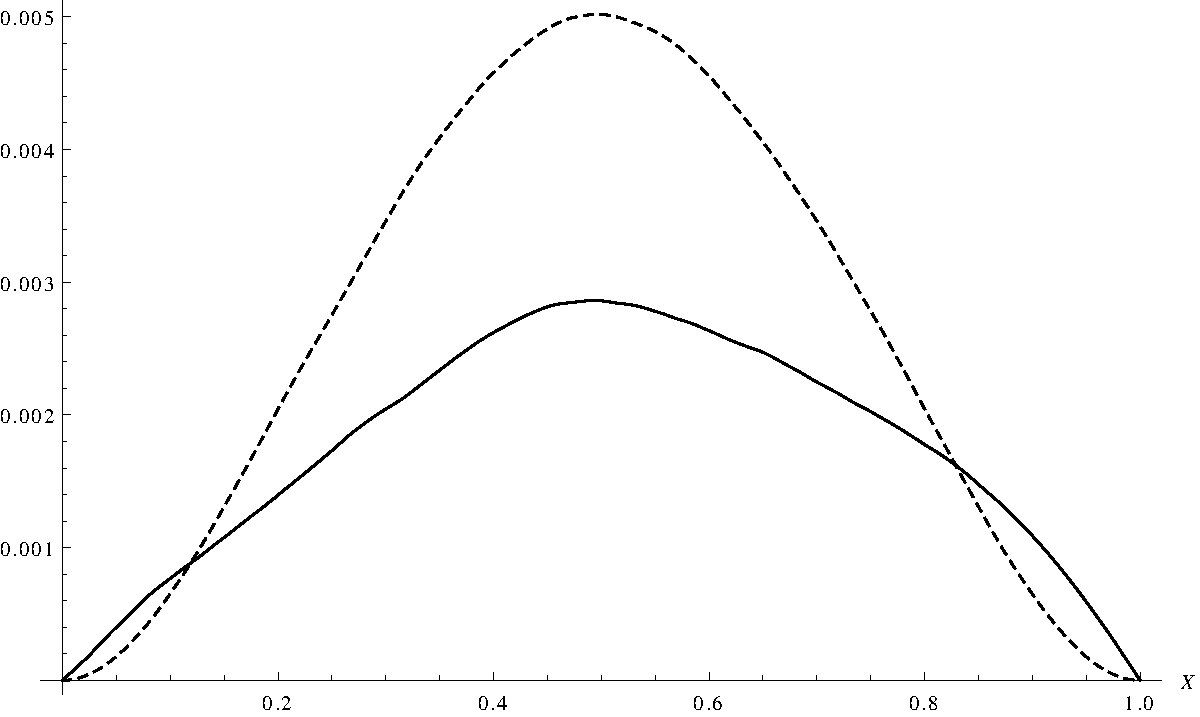
\includegraphics[width=0.9\textwidth]{continuum/figures/loc_uniform_dist/av_res_var_1000_samples}
    \caption{\label{fig:loc_uniform_1000_av_residuals}Pointwise sample mean
    (solid) and variance (dashed; scaled by \(\varepsilon^{-1}\)) of
    \(r^\varepsilon\) calculated from 1000 Monte Carlo samples for uniformly
    distributed sinks with constant (unit) strength with, \({\Pe=\varepsilon},
    {\Da=\varepsilon\Pe}\)}
\end{figure}

\FloatBarrier

\section{Sinks of varying strength}

We now allow the sinks to have different strengths. The solution between each
pair of sinks has the same form (\(C_i(x)=A_i e^{\Pe x} + B_i\)) but the
coefficients \(A_i\) and \(B_i\) will change. Let \(q_i\) be the
(nondimensional --- \(q_0\) can now be thought of as the mean sink strength
against which the strengths are nondimensionalised) strength of sink \(\xi_i\).
Going through the calculations equivalent to the above yields the following
expressions for the coefficients:
\begin{equation}
    \label{eqn:varying_strength_A_0}
    %\boxed{
    A_0 = \frac{1 -
        \frac{\Da}{\Pe} \sum_{i=1}^N q_i \left(1 - e^{\Pe(\varepsilon^{-1}
        -\xi_i)}\right)}{1 - e^{\Pe \varepsilon^{-1}}},
    %}
\end{equation}
\begin{equation}
    \label{eqn:varying_strength_B_0}
    %\boxed{
    B_0 = 1 - \frac{1 -
        \frac{\Da}{\Pe} \sum_{i=1}^N q_i \left(1 - e^{\Pe(\varepsilon^{-1}
        -\xi_i)}\right)}{1 - e^{\Pe \varepsilon^{-1}}},
    %}
    %\boxed{B_0 = 1 - \frac{1 -
    %    \frac{\Da}{\Pe} \left(\sum_{i=1}^N q_i - e^{\Pe \varepsilon^{-1}}
    %    \sum_{i=1}^{N} q_i e^{-\Pe
    %    \xi_i}\right)}{1 - e^{\Pe \varepsilon^{-1}}},}
\end{equation}
\begin{equation}
    \label{eqn:varying_strength_A_i}
    %\boxed{
    A_i = A_0 + \frac{\Da}{\Pe}\sum_{j=1}^i q_j e^{-\Pe \xi_j},
%}
\end{equation}
\begin{equation}
    \label{eqn:varying_strength_B_i}
    %\boxed{
    B_i = B_0 - \frac{\Da}{\Pe} \sum_{j=1}^i q_j.
%}
\end{equation}

\subsection{Log-normally distributed sink strengths}
If a random variable \(X\) is normally distributed, then \(Y=\exp(X)\) is
log-normally distributed, denoted by \(Y\sim\ln\mathcal{N}(\mu,\sigma^2)\). The
parameters \(\mu,\sigma^2\) are the mean and variance of the corresponding
normal distribution, \(\mathcal{N}(\mu,\sigma^2)\). They are related to the mean
\(m\) and variance \(v\) of the log-normal distribution by
\begin{gather*}
    \mu = \ln\left(\frac{m^2}{\sqrt{v+m^2}}\right)\\
    \sigma = \sqrt{\ln\left(1+\frac{v}{m^2}\right)}
\end{gather*}

\begin{figure}[ht!]
    \centering
    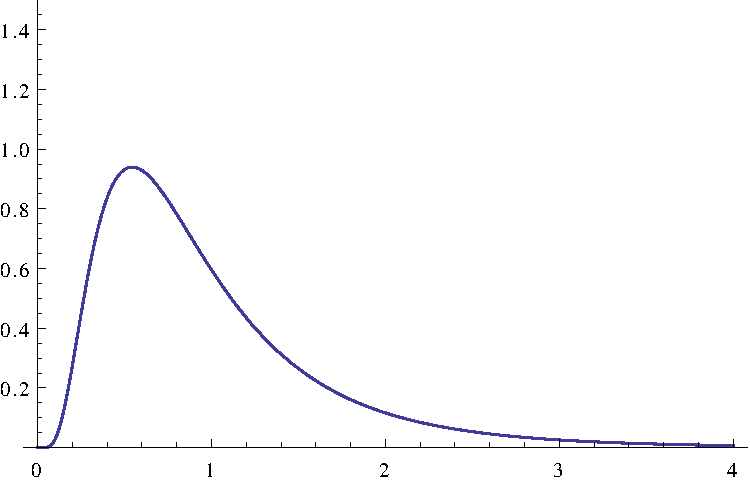
\includegraphics[width=0.7\textwidth]{continuum/figures/log_normal_pdf}
    \caption{\label{fig:log_normal_pdf}PDF of the log-normal distribution with mean 1 and variance 0.5}
\end{figure}

\FloatBarrier

\begin{figure}[ht!]
    \centering
    \begin{subfigure}[b]{0.45\textwidth}
        \centering
        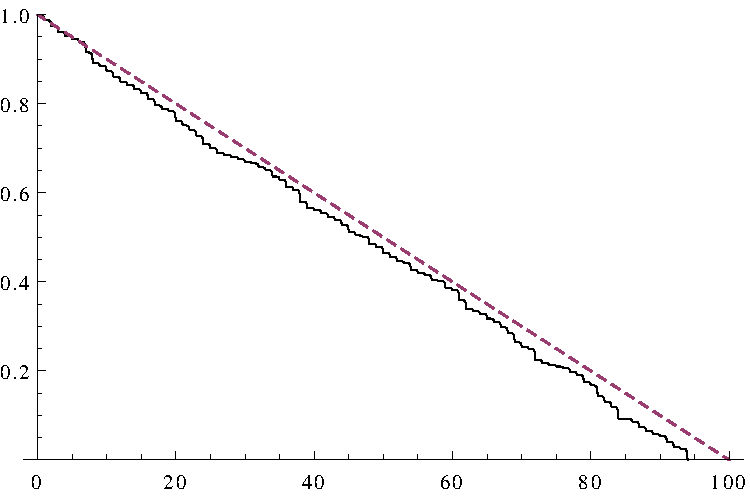
\includegraphics[scale=0.5]{continuum/figures/strength_lognormal_dist/1}
    \end{subfigure}
    \begin{subfigure}[b]{0.45\textwidth}
        \centering
        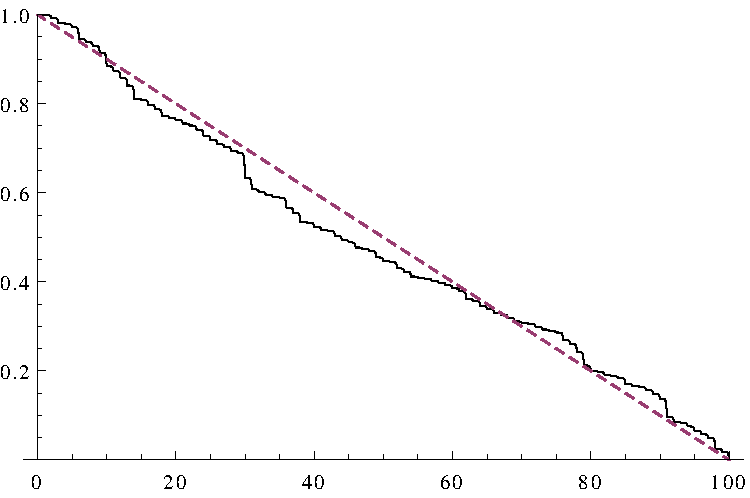
\includegraphics[scale=0.5]{continuum/figures/strength_lognormal_dist/2}
    \end{subfigure}
    \\
    \begin{subfigure}[b]{0.45\textwidth}
        \centering
        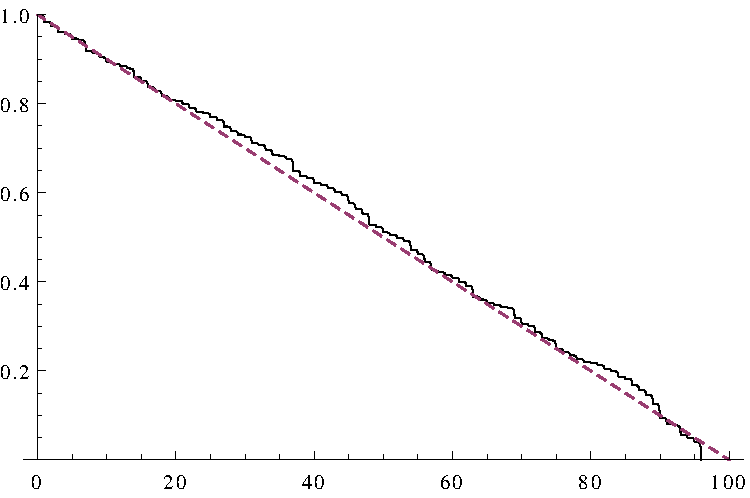
\includegraphics[scale=0.5]{continuum/figures/strength_lognormal_dist/3}
    \end{subfigure}
    \begin{subfigure}[b]{0.45\textwidth}
        \centering
        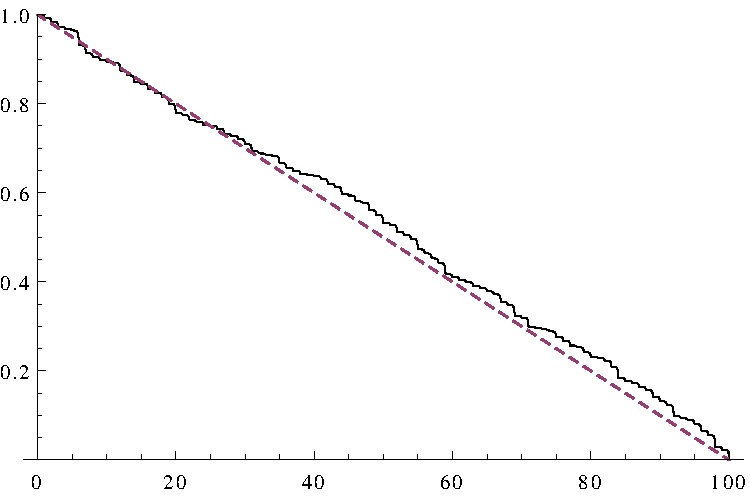
\includegraphics[scale=0.5]{continuum/figures/strength_lognormal_dist/4}
    \end{subfigure}
    \caption{\label{fig:99_sink_periodic_pos}Four realisations of 99 sinks with
    periodic positions and log-normally distributed strengths \({m=1}, {v=0.5},
    {\Pe=10}, {\Da=\varepsilon\Pe}\)}
\end{figure}

\FloatBarrier

\subsubsection{Sample statistics}

Figure~\ref{fig:log_normal_1000_av_residuals} shows the pointwise sample mean of
the residual \(r^\varepsilon = C - C^{(0)}\) for log-normally distributed sink
strengths and periodic sink positions.

%Since the mean of the log normal
%distribution used for the sink strengths is 1, one might expect (after
%performing many trials) the sample mean residuals to be close to those of the
%case of periodic sink positions and unit sink strengths. The figure, generated
%from 1000 samples, supports this.

\begin{figure}[ht!]
    \centering
    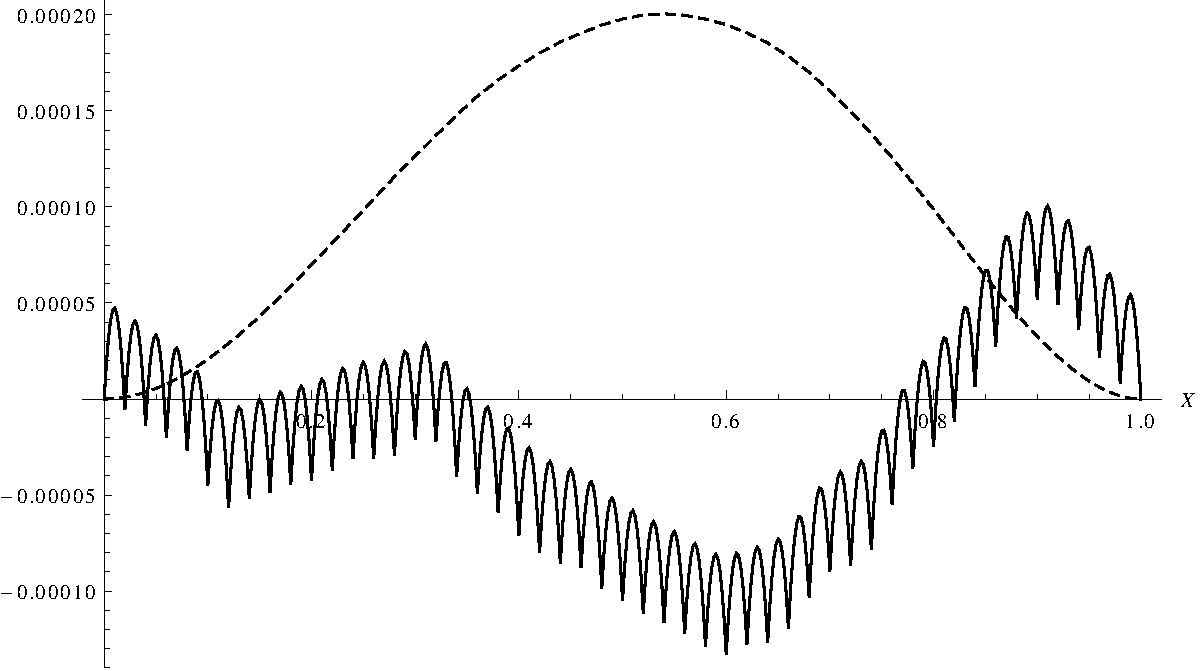
\includegraphics[width=0.9\textwidth]{continuum/figures/strength_lognormal_dist/av_res_var_1000_samples}
    \caption{\label{fig:log_normal_1000_av_residuals}Pointwise sample mean
    (solid) and variance (dashed) of \(r^\varepsilon\) calculated from
    1000 Monte Carlo samples for log-normally distributed sink strengths with
    \({m=1}, {v=0.5},
    {\Pe=\varepsilon}, {\Da=\varepsilon\Pe}\)}
\end{figure}

\FloatBarrier

\section{Homogenisation for periodically distributed sinks}

We will be applying the method of homogenisation to equations
\eqref{eqn:nondim_advec_diff} and \eqref{eqn:point_sink_dist} in the case where
the sink locations are periodically distributed, i.e. \(\xi_i = i, 1 \le i \le
N\). The motivation for this approach is the observation that there are features
of the solution \(C(x)\) that occur on different characteristic length scales.
For example, in figure~\ref{fig:99_sink_periodic_pos}, one can see that over the
length of the whole domain, there is a steady decrease in the concentration. In
addition, on the scale of the (nondimensional) distance between adjacent sinks,
\(\varepsilon\), there is a rapid change in concentration near each sink, and
the concentration then levels off until it approaches another sink. The idea of
homogenisation is to use a multiple scales expansion to capture the variations
on both length scales separately by introducing an additional variable, treated
as independent of \(x\) (technically one that tends to independence from \(x\)
as \(\varepsilon \to 0\) in a weak two-scale sense).  Then, there is usually an
averaging step over the small length scale in order to be able to extract the
approximate ``average'' behaviour over the whole domain.

We will seek solutions to \eqref{eqn:nondim_advec_diff} and
\eqref{eqn:point_sink_dist} of the form
\begin{equation}
    \label{eqn:C(x,X)}
    C(x) = \ti{C}(x,X),
\end{equation}
where we define \(X = \varepsilon x\) to be the ``slow'' variable. \(x\) is
referred to as the ``fast'' variable. The derivative with respect to \(x\)
transforms to
\begin{equation}
    \label{eqn:x_deriv_fast_slow}
    \diff{}{x} = \pdiff{}{x} + \varepsilon\pdiff{}{X},
\end{equation}
where we have ``reused'' the variable name \(x\) to simplify notation.
Henceforth, subscripts will denote partial derivatives (now that \(x\)
and \(X\) are being treated as independent).

Substituting \eqref{eqn:x_deriv_fast_slow} into
equation~\eqref{eqn:nondim_advec_diff} gives
\begin{subequations}
    \label{eqn:nondim_advec_diff_x_X}
    \begin{gather}
        \label{eqn:nondim_advec_diff_eq_x_X}
        \Pe\left(\ti{C}_x + \varepsilon\ti{C}_X\right) = \ti{C}_{xx}
        + 2\varepsilon\ti{C}_{xX} + \varepsilon^2\ti{C}_{XX} - \Da f(x),\\
        \nonumber \text{for } 0 \le x \le \varepsilon^{-1}\\
        \label{eqn:nondim_advec_diff_bcs_x_X}
        \left.\ti{C}\right|_{X=0} = 1, \quad \left.\ti{C}\right|_{X=1} = 0.
    \end{gather}
\end{subequations}
The orders of the Péclet and Damköhler numbers will therefore affect which terms
appear at each order of the problem, and so we must specify their orders before
solving. Additionally, we assume that \(\ti{C}(x,X)\) is \(x\)-periodic with
period \(1\). This represents the fact that we expect the local effect of each
sink on the concentration to be identical, so that the concentration only
depends on the position of sinks.

We can simplify this by solving only between each pair of adjacent sinks, and
introducing a condition at each sink to handle the jump in flux, so that
\(f(x)\) no longer appears explicitly:
\begin{subequations}
    \label{eqn:nondim_advec_diff_eq_x_X_no_f}
    \begin{gather}
        \Pe\left(\ti{C}_x + \varepsilon\ti{C}_X\right) = \ti{C}_{xx},
        + 2\varepsilon\ti{C}_{xX} + \varepsilon^2\ti{C}_{XX},\\
        \nonumber \text{for } x \ne i,\\
        \jump{\ti{C}_x + \varepsilon \ti{C}_X}_{x=i},\\
        \left.\ti{C}\right|_{X=0} = 1, \quad \left.\ti{C}\right|_{X=1} = 0,\\
        \nonumber i = 1, \dotsc, N.
    \end{gather}
\end{subequations}

We will seek approximate solutions to \eqref{eqn:nondim_advec_diff_eq_x_X_no_f}
of the form
\begin{equation}
    \label{eqn:x_X_asymptotic_expansion}
    C(x) = \ti{C}(x,X) = C^{(0)}(x,X) + \varepsilon C^{(1)}(x,X) + \varepsilon^2
    C^{(2)}(x,X) + \dotsb.
\end{equation}

\subsection{\(\Pe = \bo{\varepsilon}, \Da = \bo{\varepsilon^2}\)}
\label{sec:0th-order,Pe=O(e),Da=O(e^2)}

We now set \(\Pe = \varepsilon p, \Da = \varepsilon^2 q\), where \(p, q =
\bo{1}\) as \(\varepsilon \to 0\). Substituting these definitions and
\eqref{eqn:x_X_asymptotic_expansion} into
\eqref{eqn:nondim_advec_diff_eq_x_X_no_f} gives
\begin{subequations}
    \label{eqn:full_Pe=O(e),Da=O(e^2)}
    \begin{gather}
        \begin{gathered}
            p \left(
            \varepsilon C^{(0)}_x + \varepsilon^2 C^{(1)}_x + \dotsb +
            \varepsilon^2 C^{(0)}_X + \varepsilon^3 C^{(1)}_x + \dotsb \right) =
            C^{(0)}_{xx} + \varepsilon C^{(1)}_{xx} + \dotsb\\
            + 2\left(\varepsilon C^{(0)}_{xX} + \varepsilon^2 C^{(1)}_{xX} +
            \dotsb \right) +
            \varepsilon^2 C^{(0)}_{XX} + \varepsilon^3 C^{(1)}_{XX} + \dotsb,
        \end{gathered}\\
        \nonumber \text{for } x \ne i,\\
        \jump{C^{(0)}_x + \varepsilon C^{(1)}_x + \dotsb + \varepsilon C^{(0)}_X
        + \varepsilon^2 C^{(1)}_X + \dotsb}_{x=i} = \varepsilon^2 q,\\
        \left.\left(C^{(0)} + \varepsilon C^{(1)} + \dotsb\right)\right|_{X=0}
        = 1,\\
        \left.\left(C^{(0)} + \varepsilon C^{(1)} + \dotsb\right)\right|_{X=1}
        = 0,\\
        \nonumber i = 1, \dotsc, N.
    \end{gather}
\end{subequations}
We proceed by collecting terms by order in \(\varepsilon\). We also exploit the
\(x\)-periodicity of \(\ti{C}(x,X)\) by only solving in the sub-domain
\(-1/2 < x < 1/2\), representing a unit cell surrounding a sink, with the
sink at \(x = 0\). This only affects the jump conditions --- clearly
the governing equation is invariant under a translation in \(x\).

At \(\bo{1}\):
\begin{subequations}
    \label{eqn:O(1),Pe=O(e),Da=O(e^2)}
    \begin{gather}
        \label{eqn:O(1)_eqn,Pe=O(e),Da=O(e^2)}
        C^{(0)}_{xx} = 0,\\
        \label{eqn:O(1)_jump_cond,Pe=O(e),Da=O(e^2)}
        \jump{C^{(0)}}_{x=0}=0, \quad \jump{C^{(0)}_x}_{x=0}=0,\\
        \label{eqn:O(1)_bcs,Pe=O(e),Da=O(e^2)}
        \left.C^{(0)}\right|_{X=0}=1, \quad \left.C^{(0)}\right|_{X=1}=0.
    \end{gather}
\end{subequations}
Integrating \eqref{eqn:O(1)_eqn,Pe=O(e),Da=O(e^2)} gives
\begin{equation}
    \label{}
    C^{(0)}(x,X) = \ti{A}_0(X)x + \ti{B}_0(X),
\end{equation}
where \(\ti{A}_0(X),\ti{B}_0(X)\) are arbitrary functions. Since the full
domain of \(x\) is \((0,\varepsilon^{-1})\), we must suppress the first term by
setting \(\ti{A}_0 \equiv 0\). This is to avoid secular (unbounded) growth in
\(C^{(0)}\) as \(\varepsilon \to 0\). Therefore, we have that \(C^{(0) } =
C^{(0)}(X)\) only. An interpretation of this is that at a first approximation,
the behaviour of the concentration is governed solely by the boundary
conditions on the ends of the domain.

At \(\bo{\varepsilon}\):
\begin{subequations}
    \label{eqn:O(e),Pe=O(e),Da=O(e^2)}
    \begin{gather}
        \label{eqn:O(e)_eqn,Pe=O(e),Da=O(e^2)}
        C^{(1)}_{xx} = 0,\\
        \label{eqn:O(e)_jump_cond,Pe=O(e),Da=O(e^2)}
        \jump{C^{(1)}}_{x=0}=0, \quad \jump{C^{(1)}_x}_{x=0}=0,\\
        \label{eqn:O(e)_bcs,Pe=O(e),Da=O(e^2)}
        \left.C^{(1)}\right|_{X=0}=0, \quad \left.C^{(1)}\right|_{X=1}=0.
    \end{gather}
\end{subequations}
By the same reasoning as above, we find that \(C^{(1)} = C^{(1)}(X)\) only.
*Not clear on the justification for the next step* We further find that
\(C^{(1)} \equiv 0\).

At \(\bo{\varepsilon^2}\):
\begin{subequations}
    \label{eqn:O(e^2),Pe=O(e),Da=O(e^2)}
    \begin{gather}
        \label{eqn:O(e^2)_eqn,Pe=O(e),Da=O(e^2)}
        p C^{(0)}_X = C^{(2)}_{xx} + C^{(0)}_{XX},\\
        \label{eqn:O(e^2)_jump_cond,Pe=O(e),Da=O(e^2)}
        \jump{C^{(2)}}_{x=0}=0, \quad \jump{C^{(2)}_x}_{x=0}=q,\\
        \label{eqn:O(e^2)_bcs,Pe=O(e),Da=O(e^2)}
        \left.C^{(2)}\right|_{X=0}=0, \quad \left.C^{(2)}\right|_{X=1}=0.
    \end{gather}
\end{subequations}
This is the lowest order at which we have seen interaction between advection,
diffusion and uptake. We now integrate equation
\eqref{eqn:O(e^2)_eqn,Pe=O(e),Da=O(e^2)} over the unit cell:
\begin{align}
    \label{eqn:averaged_over_unit_cell,Pe=O(e),Da=O(e^2)}
    \nonumber &\left(\lim_{\delta \to 0^-} \int_{-1/2}^{\delta}\dd x +
    \lim_{\delta \to 0^+} \int_{\delta}^{1/2}\dd x\right)
    \left(p C^{(0)}_X - C^{(0)}_{XX} - C^{(2)}_{xx} \right) = 0\\
    \nonumber \implies & \left[x\right]_{-1/2}^{1/2}\left(p C^{(0)}_X -
    C^{(0)}_{XX}\right)\\
    & = p C^{(0)}_X - C^{(0)}_{XX}
    = \left.C^{(2)}_x\right|_{1/2} - \left.C^{(2)}_x\right|_{-1/2}
    -\jump{C^{(2)}_x}_{x=0}.
\end{align}
Using the assumption of periodcitiy of \(C^{(2)}_x\) in the unit cell,
equation~\eqref{eqn:averaged_over_unit_cell,Pe=O(e),Da=O(e^2)} becomes, using
the conditions~\eqref{eqn:O(e^2)_jump_cond,Pe=O(e),Da=O(e^2)}, an
advection-diffusion equation for \(C^{(0)}\):
\begin{subequations}
    \label{eqn:O(1)_averaged,Pe=O(e),Da=O(e^2)}
    \begin{gather}
        \label{eqn:O(1)_averaged_eqn,Pe=O(e),Da=O(e^2)}
        C^{(0)}_{XX} - p C^{(0)}_X = q,\\
        \label{eqn:O(1)_averaged_bcs,Pe=O(e),Da=O(e^2)}
        \left.C^{(0)}\right|_{X=0}=1, \quad \left.C^{(0)}\right|_{X=1}=0,
    \end{gather}
\end{subequations}
The solution of \eqref{eqn:O(1)_averaged,Pe=O(e),Da=O(e^2)} is
\begin{equation}
    \label{eqn:C^0(X)_solution,Pe=O(e),Da=O(e^2)}
    C^{(0)}(X) = \left(\frac{q}{p} - 1\right)\frac{e^{pX} - 1}{e^{p} - 1} -
    \frac{q}{p}X + 1
\end{equation}
Substituting \eqref{eqn:O(1)_averaged_eqn,Pe=O(e),Da=O(e^2)} into
\eqref{eqn:O(e^2)_eqn,Pe=O(e),Da=O(e^2)} gives the equation that \(C^{(2)}(X)\)
must satisfy:
\begin{equation}
    \label{eqn:O(e^2)_actual,Pe=O(e),Da=O(e^2)}
    C^{(2)}_{xx} = -q, \quad \jump{C^{(2)}}_{x=0} = 0, \quad
    \jump{C^{(2)}_x}_{x=0} = q
\end{equation}

\section{Homogenisation for randomly distributed sinks}
Similarly to the previous section, we find an approximate solution to
equation~\eqref{eqn:nondim_advec_diff} using the method of homogenisation, but
this time where the point sinks in \eqref{eqn:point_sink_dist} are now randomly
distributed.

\subsection{\(\Pe = \bo{\varepsilon}, \Da = \bo{\varepsilon^2}\)}
Again, we write \(\Pe = \varepsilon p, \Da = \varepsilon^2 q\), where \(p,q =
\bo{1}\). Starting as in the previous section, we use
equation~\eqref{eqn:x_deriv_fast_slow} to write the governing equations,
\eqref{eqn:nondim_advec_diff} and \eqref{eqn:point_sink_dist}, as

\begin{subequations}
    \label{eqn:random_sinks_full_eqns_Pe=O(e),Da=O(e^2)}
    \begin{gather}
        \label{eqn:random_sinks_full_eqns_Pe=O(e),Da=O(e^2)_eq}
        \ti{C}_{xx} + 2\varepsilon\ti{C}_{xX} + \varepsilon^2\ti{C}_{XX}
        - \varepsilon p\left(\ti{C}_x + \ti{C}_X\right) = \varepsilon^2 q f,\\
        \label{eqn:random_sinks_full_eqns_Pe=O(e),Da=O(e^2)_bcs}
        \left.\ti{C}\right|_{X=0} = 1, \quad \left.\ti{C}\right|_{X=1} = 0.
    \end{gather}
\end{subequations}

We again introduce the asymptotic expansion \eqref{eqn:x_X_asymptotic_expansion}
and substitute this into
equation~\eqref{eqn:random_sinks_full_eqns_Pe=O(e),Da=O(e^2)} to obtain
\begin{subequations}
    \label{eqn:random_sinks_expanded_Pe=O(e),Da=O(e^2)}
    \begin{gather}
        \label{eqn:random_sinks_expanded_Pe=O(e),Da=O(e^2)_eq}
        \begin{gathered}
            C^{(0)}_{xx} + \varepsilon C^{(1)}_{xx} + \dotsb +
            2\left(\varepsilon C^{(0)}_{xX} + \varepsilon^2 C^{(1)}_{xX} +
            \dotsb\right) + \varepsilon^2 C^{(0)}_{XX} + \varepsilon^3
            C^{(1)}_{XX} + \dotsb\\
            - p\left(\varepsilon C^{(0)}_x + \varepsilon^2 C^{(1)}_x + \dotsb +
            \varepsilon^2 C^{(0)}_X + \varepsilon^3 C^{(1)}_X + \dotsb \right) =
            \varepsilon^2 q f
        \end{gathered}\\
        \label{eqn:random_sinks_expanded_Pe=O(e),Da=O(e^2)_bc_X=0}
        \left.\left(C^{(0)} + \varepsilon C^{(1)} + \dotsb
        \right)\right|_{X=0}=1\\
        \label{eqn:random_sinks_expanded_Pe=O(e),Da=O(e^2)_bc_X=1}
        \left.\left(C^{(0)} + \varepsilon C^{(1)} + \dotsb
        \right)\right|_{X=1}=0
    \end{gather}
\end{subequations}

We proceed by collecting terms by their order in \(\varepsilon\).

At \(\bo 1\):
\begin{subequations}
    \label{eqn:random_sinks_O(1),Pe=O(e),Da=O(e^2)}
    \begin{gather}
        \label{eqn:random_sinks_O(1)_eqn,Pe=O(e),Da=O(e^2)}
        C^{(0)}_{xx} = 0,\\
        \label{eqn:random_sinks_O(1)_bcs,Pe=O(e),Da=O(e^2)}
        \left.C^{(0)}\right|_{X=0}=1, \quad \left.C^{(0)}\right|_{X=1}=0.
    \end{gather}
\end{subequations}
Integrating \eqref{eqn:random_sinks_O(1)_eqn,Pe=O(e),Da=O(e^2)} gives
\begin{equation}
    \label{}
    C^{(0)}(x,X) = \ti{A}_0(X)x + \ti{B}_0(X),
\end{equation}
where \(\ti{A}_0(X),\ti{B}_0(X)\) are arbitrary functions. As before, we must
set \(\ti{A}_0 \equiv 0\) and so we have that \(C^{(0)} = C^{(0)}(X)\).

At \(\bo \varepsilon\):
\begin{subequations}
    \label{eqn:random_sinks_O(e),Pe=O(e),Da=O(e^2)}
    \begin{gather}
        \label{eqn:random_sinks_O(e)_eqn,Pe=O(e),Da=O(e^2)}
        C^{(1)}_{xx} = 0,\\
        \label{eqn:random_sinks_O(e)_bcs,Pe=O(e),Da=O(e^2)}
        \left.C^{(1)}\right|_{X=0}=0, \quad \left.C^{(1)}\right|_{X=1}=0.
    \end{gather}
\end{subequations}
Again, we obtain the same at this order as in the periodic case: \(C^{(1)} =
C^{(1)}(X)\).

At \(\bo{\varepsilon^2}\):
\begin{subequations}
    \label{eqn:random_sinks_O(e^2),Pe=O(e),Da=O(e^2)}
    \begin{gather}
        \label{eqn:random_sinks_O(e^2)_eqn,Pe=O(e),Da=O(e^2)}
        C^{(2)}_{xx} = q\left(f(x) - F(X)\right)\\
        \label{eqn:random_sinks_O(e^2)_bcs_C^1,Pe=O(e),Da=O(e^2)}
        \left.C^{(1)}\right|_{x=0} = 0, \quad
        \left.C^{(1)}\right|_{x=\varepsilon^{-1}} = 0,\\
        \label{eqn:random_sinks_O(e^2)_bcs_C^2,Pe=O(e),Da=O(e^2)}
        \left.C^{(2)}\right|_{x=0} = 0, \quad
        \left.C^{(2)}\right|_{x=\varepsilon^{-1}} = 0,
    \end{gather}
\end{subequations}
where
\begin{equation}
    \label{eqn:F(X)_Pe=O(e),Da=O(e^2)}
    F(X) = \frac{1}{q}\left(C^{(0)}_{XX} - pC^{(0)}_X\right).
\end{equation}
Define \(xi_0 = 0, \xi_{N+1} = \varepsilon^{-1}\) for convenience. Then
integrating equation~\eqref{eqn:random_sinks_O(e^2)_eqn,Pe=O(e),Da=O(e^2)} twice
gives
\begin{gather*}
    C^{(2)}_x = q \int_{x_0}^x \Big[f(s) - F(X)\Big] \dd s = -q F(X)(x-x_0)
    + \alpha_i(X)\\
    \implies C^{(2)}(x,X) = \int_{x_0}^x \Big[-q F(X)(s-x_0) +
    \alpha_i(X)\Big] \dd s\\
    =-\frac{1}{2} q F(X)(x-x_0)^2 + \alpha_i(X)(x-x_0) +
    \beta_i(X),
\end{gather*}
for \(\xi_i < x < \xi_{i+1}\), where the \(\alpha_i(X), \beta_i(X)\) are
arbitrary functions of \(X\), and \(x_0\) is an arbitrary constant. Taking \(x_0
= \xi_i\) and absorbing the extra constant terms into the definition of
\(\alpha_i\) and \(\beta_i\), we obtain
\begin{equation}
    \label{eqn:random_sinks_C^2_alpha_beta_i_Pe=O(e)_Da=O(e^2)}
    C^{(2)}(x,X) = -\frac{1}{2} q F(X)(x-\xi_i)^2 + \alpha_i(X)(x-\xi_i) +
    \beta_i(X),
\end{equation}
for \(\xi_i < x < \xi_{i+1}\).

TODO type out details of finding \(\alpha_i, \beta_i\).

To simplify the expressions that will follow, we make these definitions:
\begin{gather}
    \Delta_i = \xi_i - \xi_{i-1},\\
    \left(R_i,S_i,T_i,U_i\right) = \sum_{j=1}^i
    \left(\xi_j,\Delta_j^2,\xi_j\Delta_j,\xi_j^2\right),
\end{gather}
for \(i=1,\dotsc,N+1\).
Then
\begin{subequations}
    \label{eqn:alpha_beta_i_recursive}
    \begin{gather}
        \label{eqn:alpha_i_recursive}
        \alpha_i=\alpha_{i-1} + q\left(1-F\Delta_i\right),\\
        \label{eqn:beta_i_recursive}
        \beta_i=\beta_{i-1} - \frac{1}{2} q F \Delta_i^2 + \alpha_{i-1}\Delta_i.
    \end{gather}
\end{subequations}

Looking at
equation~\eqref{eqn:random_sinks_C^2_alpha_beta_i_Pe=O(e)_Da=O(e^2)}, it is
clear that to satisfy the condition \(\left.C^{(2)}\right|_{x=0} = 0\), we must
have \(\beta_0 = 0\). Now, if we make the assumption that \(F\) is constant,
which in turn implies that the \(\alpha_i,\beta_i\) are constants, then
\(\alpha_i, \beta_i\) can be expressed as (TODO type out details)
\begin{subequations}
    \label{eqn:alpha_beta_i_F_const}
    \begin{gather}
        \label{eqn:alpha_i_F_const}
        \alpha_i=\alpha_0 + q(i + F\xi_i),\\
        \label{eqn:beta_i_F_const}
        \beta_i=-\frac{1}{2} q F S_i + \alpha_{0}\xi_i + q \sum_{j=1}^i
        \Delta_j\left(j - 1 - F\xi_{j-1}\right).
    \end{gather}
\end{subequations}

Substituting these expressions for \(\alpha_i, \beta_i\) into
equation~\eqref{eqn:random_sinks_C^2_alpha_beta_i_Pe=O(e)_Da=O(e^2)} gives
\begin{equation}
    \label{eqn:random_sinks_C^2_Pe=O(e)_Da=O(e^2)}
    C^{(2)} = -\frac{1}{2} q F x^2 + \alpha_0 x + q(ix - R_i).
\end{equation}

We now impose the condition \(\left.C^{(2)}\right|_{x=\varepsilon^{-1}}=0\)
from \eqref{eqn:random_sinks_O(e^2)_bcs_C^2,Pe=O(e),Da=O(e^2)} on
\eqref{eqn:random_sinks_C^2_Pe=O(e)_Da=O(e^2)} to find \(\alpha_0\):
\begin{align*}
    &\left.C^{(2)}\right|_{x=\varepsilon^{-1}} = -\frac{1}{2}q F
    \varepsilon^{-2} + \alpha_0\varepsilon^{-1} + q\left(N\varepsilon^{-1} -
    R_N\right) = 0\\
    \implies & \alpha_0 = \frac{1}{2}q F \varepsilon^{-1} - q\left(N -
    \varepsilon R_N\right).
\end{align*}
Substituting this back into \eqref{eqn:random_sinks_C^2_Pe=O(e)_Da=O(e^2)}
gives the relationship between the sink locations and the
\(\bo{\varepsilon^2}\) fluctuations of the solute distribution:
\begin{equation}
    \label{eqn:random_sinks_C^2_final_Pe=O(e)_Da=O(e^2)}
    C^{(2)}(x) = \frac{1}{2} q F x(\varepsilon^{-1} - x) +
    q\left(x\left(\varepsilon R_N + i - N \right) - R_i\right),
\end{equation}
for \(\xi_i < x < \xi_{i+1}\).

\subsubsection{\(f=f_n\) --- normally perturbed sink positions}
We concentrate on the case \(f = f_n\) in order to exploit useful properties of
normal distributions. In this case, we have \(\xi_i \sim
\mathcal{N}(i,\sigma^2)\) --- a normal distribution with mean \(i\) and
variance \(\sigma^2\). By considering the definition of a general normal
distribution \(f(x)\) in terms of the standard normal distribution \(\phi(x)\),
\begin{gather*}
    f(x) = \frac{1}{\sigma}\phi\left(\frac{x-\mu}{\sigma}\right),\\
    \text{where}\quad \phi(x) = \frac{1}{\sqrt{2\pi}}e^{-\frac{1}{2}x^2},
\end{gather*}
and by using standard properties of the expected value and variance,
we can write \(\xi_i \sim \mathcal{N}(i,\sigma^2) \sim i + \sigma
\mathcal{N}(0,1)\). In \eqref{eqn:random_sinks_C^2_final_Pe=O(e)_Da=O(e^2)},
the randomness is introduced solely through the appearance of \(R_i\) and
\(R_N\). Therefore, to analyse the distribution of the fluctuations in terms
of the distribution of the sinks, we need only consider terms involving these
quantities, namely \(\varepsilon x R_N - R_i\). The perturbations of each
sink's position about its mean are taken to be independent, so that we can
sum the distribution to obtain another normal distribution. Setting \(x =
X/\varepsilon\) (what's the justification for this? They are independent!):
\begin{align*}
    X R_N - R_i &= X \sum_{j=1}^N \xi_j - \sum_{j=1}^i \xi_j = X
    \left(\sum_{j=1}^i \xi_j + \sum_{j=i+1}^N \xi_j\right) - \sum_{j=1}^i
    \xi_j\\
    &=(X-1)\sum_{j=1}^i \xi_j + X\sum_{j=i+1}^N \xi_j\\
    &\sim (X-1)\sum_{j=1}^i \mathcal{N}(j,\sigma^2) + X\sum_{j=i+1}^N
    \mathcal{N}(j,\sigma^2)\\
    &\sim
    (X-1)\mathcal{N}\left(\tfrac{1}{2}i(i+1),i\sigma^2\right) + X
    \mathcal{N}\left(\tfrac{1}{2}N(N+1) -
    \tfrac{1}{2}i(i+1),(N-i)\sigma^2\right)\\
    &\sim \mathcal{N}\left(\tfrac{1}{2}i(i+1)(X-1),
    i\sigma^2(X-1)^2\right)\\
    &\quad + \mathcal{N}\left(\tfrac{1}{2}N(N+1)X -
    \tfrac{1}{2}i(i+1)X, \sigma^2(N-i)X^2\right)\\
    & \sim \mathcal{N}\left(\tfrac{1}{2}N(N+1)X - \tfrac{1}{2}i(i+1),
    \sigma^2\left[i(X-1)^2 + (N-i)X^2\right]\right),
\end{align*}
where we have used standard properties of normal distributions.

Then write \(i = (X/\varepsilon) + (i - x)\) and substitute.

% TODO finish this section!!! It should be well ease --- just do what Oliver was
% writing on the board...

\section{First-order kinetics}

So far, we have only consider the case of zero-th order kinetics, where the
sink function \(f(x)\) was independent of the concentration profile \(C(x)\).
Now we consider the case where sink function is given by \(f(x) C(x)\). The
boundary conditions on the concentration remain the same, and so the full
set of equations is
\begin{subequations}
    \label{eqn:nondim_advec_diff_1st_order}
    \begin{gather}
        \label{eqn:nondim_advec_diff_1st_order_eq}
        C_{xx} - \Pe C_x = \Da f(x) C(x), \text{ for } 0 < x < \varepsilon^{-1},\\
        \label{eqn:nondim_advec_diff_1st_order_bcs}
        C(0) = 1, \quad C(\varepsilon^{-1}) = 0,\\
        \label{eqn:nondim_advec_diff_1st_order_sinks}
        f(x) = \sum_{i=1}^N \delta(x-\xi_i).
    \end{gather}
\end{subequations}

\subsection{Exact solution}

\subsection{Homogenisation}
In this section we describe the procedure involved in deriving the approximate
solution of the system \eqref{eqn:nondim_advec_diff_1st_order} by the method of
homogenisation.

As before, we begin by introducing the variable \(X = \varepsilon x\), and
writing the \(x\)-derivatives as \eqref{eqn:x_deriv_fast_slow}. We then seek
solutions of the form \(C(x) = \ti{C}(x,X)\), and introduce the asymptotic
expansion in \eqref{eqn:x_X_asymptotic_expansion}. We must now make assumptions
about the orders of \(\Pe\) and \(\Da\) to be able to proceed.

\subsubsection{\(\Pe = \bo{\varepsilon}, \Da = \bo{\varepsilon^2}\)}
Following section~\ref{sec:0th-order,Pe=O(e),Da=O(e^2)}, we now set \(\Pe =
\varepsilon p, \Da = \varepsilon^2 q\), where \(p, q = \bo{1}\) as \(\varepsilon
\to 0\). Using these assumptions, and those given in the previous paragraph,
equation \eqref{eqn:nondim_advec_diff_1st_order} becomes
\begin{subequations}
    \label{eqn:full_1st-order,Pe=O(e),Da=O(e^2)}
    \begin{gather}
        \label{eqn:full_1st-order,Pe=O(e),Da=O(e^2)_eq}
        \begin{gathered}
            p \left(
            \varepsilon C^{(0)}_x + \varepsilon^2 C^{(1)}_x + \dotsb +
            \varepsilon^2 C^{(0)}_X + \varepsilon^3 C^{(1)}_x + \dotsb \right) =
            C^{(0)}_{xx} + \varepsilon C^{(1)}_{xx} + \dotsb\\
            + 2\left(\varepsilon C^{(0)}_{xX} + \varepsilon^2 C^{(1)}_{xX} +
            \dotsb \right) +
            \varepsilon^2 C^{(0)}_{XX} + \varepsilon^3 C^{(1)}_{XX} + \dotsb,
        \end{gathered}\\
        \nonumber \text{for } x \ne i,\\
        \label{eqn:full_1st-order,Pe=O(e),Da=O(e^2)_jump_cond}
        \jump{C^{(0)}_x + \varepsilon C^{(1)}_x + \dotsb + \varepsilon C^{(0)}_X
        + \varepsilon^2 C^{(1)}_X + \dotsb}_{x=i} = q\left(\varepsilon^2 C^{(0)}
        + \varepsilon^3 C^{(1)} + \dotsb\right),\\
        \left.\left(C^{(0)} + \varepsilon C^{(1)} + \dotsb\right)\right|_{X=0}
        = 1,\\
        \left.\left(C^{(0)} + \varepsilon C^{(1)} + \dotsb\right)\right|_{X=1}
        = 0,\\
        \nonumber i = 1, \dotsc, N.
    \end{gather}
\end{subequations}
It is apparent that the only change when compared to the zero-th order case
\eqref{eqn:full_Pe=O(e),Da=O(e^2)} is the jump condition
\eqref{eqn:full_1st-order,Pe=O(e),Da=O(e^2)_jump_cond} which now depends on the
concentration, with a non-zero contribution first at \(\bo{\varepsilon^2}\).
Since the jump in concentration flux is zero at \(\bo{1}\) and
\(\bo{\varepsilon}\), the same as the zero-th order kinetics problem, we again
obtain equations \eqref{eqn:O(1),Pe=O(e),Da=O(e^2)} and
\eqref{eqn:O(e^2),Pe=O(e),Da=O(e^2)} at these orders, respectively. Therefore,
we have \(C^{(0)} = C^{(0)}(X)\) and \(C^{(1)} \equiv 0\). At the next order,
however, the system will be different.

At \(\bo{\varepsilon^2}\):
\begin{subequations}
    \label{eqn:1st-order,O(e^2),Pe=O(e),Da=O(e^2)}
    \begin{gather}
        \label{eqn:1st-order,O(e^2)_eqn,Pe=O(e),Da=O(e^2)}
        p C^{(0)}_X = C^{(2)}_{xx} + C^{(0)}_{XX},\\
        \label{eqn:1st-order,(e^2)_jump_cond,Pe=O(e),Da=O(e^2)}
        \jump{C^{(2)}}_{x=0}=0, \quad \jump{C^{(2)}_x}_{x=0}=q C^{(0)},\\
        \label{eqn:1st-order,(e^2)_bcs,Pe=O(e),Da=O(e^2)}
        \left.C^{(2)}\right|_{X=0}=0, \quad \left.C^{(2)}\right|_{X=1}=0.
    \end{gather}
\end{subequations}
As previously, we integrate over a unit cell, \(-1/2 < x < 1/2\), to obtain the
governing equation for \(C^{(0)}(X)\) with the appropriate boundary conditions:
\begin{subequations}
    \label{eqn:1st-order,C^(0)_system}
    \begin{gather}
        C^{(0)}_{XX} - p C^{(0)}_X = q C^{(0)},\\
        \left.C^{(0)}\right|_{X=0} = 1, \quad \left.C^{(0)}\right|_{X=1}=0
    \end{gather}
\end{subequations}

The solution to \eqref{eqn:1st-order,C^(0)_system} is
\begin{equation}
    \label{eqn:1st-order,C^(0)_solution}
    C^{(0)}(X) = \frac{e^{pX/2}\sinh\left( \sqrt{q+p^2/4}
(1-X)\right)}{\sinh\left( \sqrt{q+p^2/4} \right)}
\end{equation}
